\chapter{State Feedback}
\label{state_feedback}

The state, $x(t)$, of a dynamical system is a collection of variables that permits prediction
of the future development of a system. In this chapter we want to  explore the idea of designing
the dynamics of a system through feedback of the state.  A typical feedback control system with state feedback
is shown in figure \ref{state_feedback_sys}

\begin{figure}[!htb]
\begin{center}
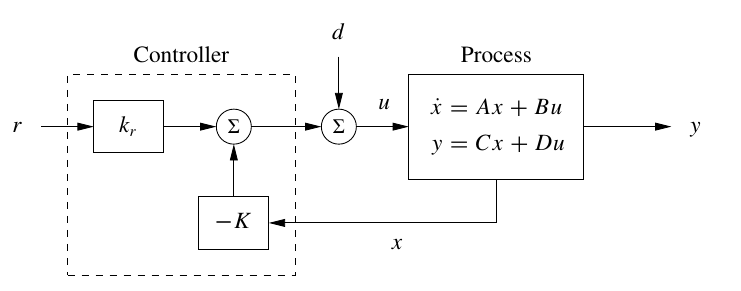
\includegraphics[scale=0.280]{img/state_feedback/state_feedback_sys.jpeg}
\end{center}
\caption{A feedback control system with state feedback. The controller uses the system
state $x$ and the reference input $r$ to command the process through its input $u$. We model
disturbances via the additive input $d$.}
\label{state_feedback_sys}
\end{figure}


The goal of the feedback controller is to regulate the output of the system $y$ such that it tracks the reference input in the presence of disturbances and also uncertainty in the process dynamics.

\section{Overview}
We have already mentioned the general form of the state-space model is 

\begin{eqnarray}
\dot{x} = f(x, u, d) \\
y = h(x,u,d)
\end{eqnarray}

both $f$ and $h$ can be nonlinear functions of their arguments however in this section we will assume that we are dealing with a linear system. Our aim is
to design a state feedback controller. Thus, let's consider again the system

\begin{eqnarray}
\dot{x} = Ax + Bu \\
y = Cx + Du
\end{eqnarray}

The poles of the system are given by the eigenvalues of the matrix $A$ which are the roots of the characteristic polynomial

\begin{equation}
det(sI-A) = 0
\end{equation}

Feedback control is a method for shaping the dynamics of the system. This is done by modifying the eigenvalues of the system using the input $u$. Indeed, let's assume that $u$
can be written as 

\begin{equation}
u = -Kx + K_r r
\end{equation}

with $K \in r^{p\times n}$, $k_r \in R^{p\times r}$ and $r \in R^r$ is the reference input. We can shape the dynamics of the system via the feedback gain $K$. $K_r$ is used to change the steady state level
of the system. The system dynamics becomes

\begin{eqnarray}
\dot{x} = Ax + B(-Kx + K_r r) \\
 = (A-BK)x + BK_r r
\end{eqnarray}

The control objective now is to choose $K$ such that the closed loop dynamics $A-BK$ get the desired properties.



\begin{framed}
\theoremstyle{remark}
\begin{remark}{\textbf{Steady state reference gain}}

The steady-state reference gain $K_r$ does not affect the stability of the system but it does affect the steady state solution.
\end{remark}
\end{framed}


The gain $K_r$ is chosen such that 

\begin{equation}
y(t) \approx r(t), ~~ \text{as} ~~ t \rightarrow \infty
\end{equation}

At steady state

\begin{equation}
\dot{x} = 0 
\end{equation}

thus we can write


\begin{eqnarray}
0 = (A-BK)x + BK_r r \\
y = Cx 
\end{eqnarray}


Hence, we can write for the output $y$


\begin{equation}
y = -C(A-Bk)^{-1}BK_r r 
\end{equation}

If we want $y(t) \approx r(t)$, as $ t \rightarrow \infty$, then $K_r$ should be chosen as

\begin{equation}
K_r = - ( C(A-BK)^{-1}B)^{-1} 
\end{equation}

The design of the controller becomes a two step process.

\begin{itemize}

\item shape the dynamics by choosing $K$
\item set the steady-state level by choosing $K_r$
\end{itemize}

This way the reference gain depends on the feedback gain. Using the steady-state feedback gain $K_r$ we can achieve zero steady-state error but this depends on the model parameters also. Integration can be used in order to remove the steady-state error. This can be done by introducing a new variable to remove the steady-state error:

We will illustrate how  this is done assuming a SISO system. 

\begin{equation}
\dot{z}(t) = y(t) - r(t)
\end{equation}

The new state-space model becomes


\begin{equation}
\begin{bmatrix}
 \dot{x} \\
 \dot{z} 
\end{bmatrix} = 
\begin{bmatrix}
 Ax-Bu \\
 y-r 
\end{bmatrix} = 
\begin{bmatrix}
 Ax-Bu \\
 Cx-r  
\end{bmatrix}
\end{equation}


the above can be written as

\begin{equation}
\begin{bmatrix}
 A & 0 \\
 0 & 0 
\end{bmatrix} +  
\begin{bmatrix}
 B \\
 0 
\end{bmatrix}u +
\begin{bmatrix}
 0 \\
 -1  
\end{bmatrix}r
\end{equation}

Thus, the new controller now becomes

\begin{equation}
u(t) = - Kx(t) - K_I z(t) + K_r r(t)
\end{equation}

\section{Reachability}
One of the fundamental properties of a control system is what set of points in the
state space can be reached through the choice of a control input. It turns out that the
property of reachability is also fundamental in understanding the extent to which
feedback can be used to design the dynamics of a system.

\begin{framed}
\theoremstyle{definition}
\begin{definition}{Reachability}

A linear system is reachable if for any $x_0, x_f \in R^n$ there exists a $T > 0$ and $u: [0,T] \rightarrow R$ such tha the corresponding solution satisfies $x(0) = x_0$ and $x(T) = x_f$.
\end{definition}
\end{framed}


\begin{figure}[!htb]
\begin{center}
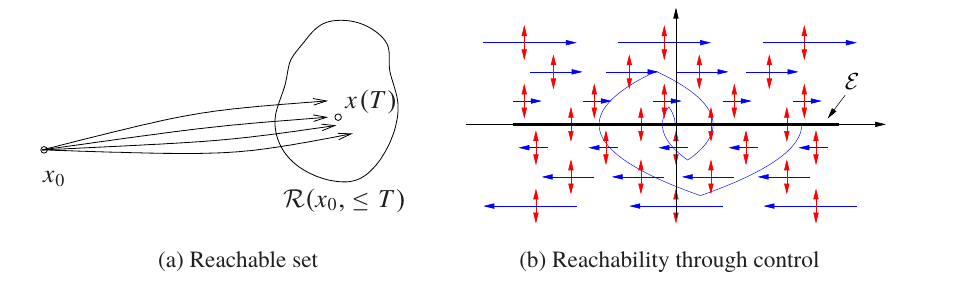
\includegraphics[scale=0.280]{img/state_feedback/reachability.jpeg}
\end{center}
\caption{The reachable set for a control system. The set $R(x_0,\leq T )$ shown in (a) is the set
of points reachable from $x_0$ in time less than $T$ . The phase portrait in (b) shows the dynamics
for a double integrator, with the natural dynamics drawn as horizontal arrows and the control
inputs drawn as vertical arrows. The set of achievable equilibrium points is the $x$ axis. By
setting the control inputs as a function of the state, it is possible to steer the system to the
origin, as shown on the sample path.}
\label{reachability}
\end{figure}


The definition of reachability addresses whether it is possible to reach all points
in the state space in a transient fashion. In many applications, the set of points that
we are most interested in reaching is the set of equilibrium points of the system
(since we can remain at those points once we get there). The set of all possible
equilibria for constant controls is given by:

\begin{equation}
E = { x_e: Ax_e + Bu_e = 0 ~~ \text{for some} ~~ u_e \in R }
\end{equation}

To find general conditions under which a linear system is reachable, we will
first give a heuristic argument based on formal calculations with impulse functions.

\begin{framed}
\theoremstyle{remark}
\begin{remark}{Equilibrium points and reachability}

We note that if we can reach all points in the state space through some choice of
input, then we can also reach all equilibrium points.
\end{remark}
\end{framed}

\subsection{Testing for reachability with impulse functions}

When the initial state is zero, the resppnse of the system to an input $u(t)$ is given by

\begin{equation}
x(t) = \int_{0}^{t} e^{A(t-\tau)}Bu(\tau)d\tau
\end{equation}

Let's choose the input to be an impulse function $\delta(t)$. The state then becomes

\begin{framed}
\theoremstyle{remark}
\begin{remark}{Impulse function $\delta(t)$}

\end{remark}
\end{framed}

\begin{equation}
x_{\delta}  = \int_{0}^{t} e^{A(t-\tau)}Bu(\tau)d\tau = \frac{dx_s}{dt} = e^{At}B
\end{equation}

(Note that the state changes instantaneously in response to the impulse.) We can
find the response to the derivative of an impulse function by taking the derivative
of the impulse response (Exercise 5.1):

\begin{equation}
\frac{dx_{\delta}}{dt} = Ae^{At}B
\end{equation}

Continuing this process and using the linearity of the system, the input

\begin{equation}
u(t) = \alpha_1\delta(t) + \alpha_2 \frac{d\delta(t)}{dt} + \dots +  \alpha_n \frac{d^{n-1}\delta(t)}{dt^{n-1}}  
\end{equation}

gives the state

\begin{equation}
x(t) = \alpha_1e^{At}B + \alpha_2Ae^{At}B + \dots +  \alpha_n A^{n-1}e^{At}B  
\end{equation}

On the right is a linear combination of the columns of the matrix

\begin{equation}
W_r = \begin{bmatrix}
 B & AB & \ldots & A^{n-1}B 
\end{bmatrix}
\end{equation}

To reach an arbitrary point  in the state  space,  we  thus  require that there are $n$ linear independent columns of the matrix $W_r$. 

\begin{framed}
\theoremstyle{remark}
\begin{remark}{\textbf{The reachability matrix $W_r$}}

The matrix $W_r$ is called the reachability
matrix.

\end{remark}
\end{framed}

\subsection{Testing for reachability with the convolution equation}

However, an input $u(t)$ consisting of a sum of impulse functions and their derivatives is a very
violent signal. To see that an arbitrary point can be reached with smoother signals we can make use of the convolution equation. Assuming that the initial condition is zero, the state of a linear system is given by
\begin{equation}
x(t)  = \int_{0}^{t} e^{A(t-\tau)}Bu(\tau)d\tau = \int_{0}^{t} e^{A(\tau)}Bu(t-\tau)d\tau
\end{equation}

It follows from the theory of matrix functions, specifically the Cayley-Hamilton
theorem (see Exercise 6.10), that


\begin{framed}
\theoremstyle{remark}
\begin{remark}{The Cayley-Hamilton theorem}

\end{remark}
\end{framed}

\begin{equation}
e^{A\tau}  = I\alpha_0(\tau) + A\alpha_1(\tau) + \dots + A^{n-1}\alpha_{n-1}(\tau)
\end{equation}

where $\alpha_i$ are scalar functions, and we find that 

\begin{equation}
x(t)  = B\int_{0}^{t} \alpha_0(\tau)u(t-\tau)d\tau + AB\int_{0}^{t} \alpha_1(\tau)u(t-\tau)d\tau+ \dots + A^{n-1}B\int_{0}^{t} \alpha_{n-1}(\tau)u(t-\tau)d\tau  
\end{equation}

Again we observe that the right-hand side is a linear combination of the columns
of the reachability matrix $W_r$ given by equation (6.3). This basic approach leads to
the following theorem.

\begin{framed}
\theoremstyle{theorem}
\begin{theorem}{Reachability rank condition}

 A linear system is reachable if and
only if the reachability matrix $W_r$ is invertible.
\end{theorem}
\end{framed}


\subsection{Reachable Canonical Form}

It is often convenient to change coordinates and write the dynamics of the system in the transformed coordinates

\begin{equation}
z = Tx
\end{equation}

One application of a change of coordinates is to convert a system into a
canonical form in which it is easy to perform certain types of analysis.

\begin{framed}
\theoremstyle{remark}
\begin{remark}{\textbf{Reachable Canonical Form}}

A linear state space system is in reachable canonical form, if its dynamics are given by

\begin{eqnarray}
\frac{dz}{dt} = Az + Bu \\
y=Cz + du
\end{eqnarray}

\end{remark}
\end{framed}

The characteristic polynomial for a system in reachable canonical form is given

\begin{equation}
\lambda(s) = s^n +\alpha_1s^{n-1}+ \dots + \alpha_{n-1}s + \alpha_n
\end{equation}

The reachability matrix also has a relatively simple structure:

We now consider the problem of changing coordinates such that the dynamics
of a system can be written in reachable canonical form. Let $A$, $B$ represent the
dynamics of a given system and $\tilde{A}, \tilde{B}$ be the dynamics in reachable canonical form.
Suppose that we wish to transform the original system into reachable canonical
form using a coordinate transformation $z = Tx$. As shown in the last chapter, the
dynamics matrix and the control matrix for the transformed system are

\begin{equation}
\tilde{A} = TAT^{-1}, ~~ \tilde{B} = TB
\end{equation}

The reachability matrix for the transformed system then becomes

\begin{equation}
\tilde{W}_r = \begin{bmatrix}
 \tilde{B} & \tilde{A}\tilde{B} & \ldots & \tilde{A}^{n-1}\tilde{B} 
\end{bmatrix}
\end{equation}

We can transforming each element individually and thus get the reachability matrix fro the transformed system

\begin{equation}
\tilde{W}_r = TW_r
\end{equation}

However, we know that $W_r$ is invertible. Therefore we can solve for the transformation $T$ that takes the system into reachable canonical form:

\begin{equation}
T = \tilde{W}_r W_{r}^{-1}
\end{equation}


\begin{framed}
\theoremstyle{theorem}
\begin{theorem}{Reachable canonical form}

Let $A$ and $B$ be the dynamics and control matrices for a reachable system. Then there exists a transformation

\begin{equation}
z = Tx \nonumber
\end{equation}

such that in the transformed coordinates  the dynamics and control matrices are in the reachable 
canoinical form and the characteristic polynomial for $A$ is given by

\begin{equation}
\text{det}(sI-A) = 0 \nonumber
\end{equation}

\end{theorem}
\end{framed}

One important implication of this theorem is that for any reachable system, we
can assume without loss of generality that the coordinates are chosen such that the
system is in reachable canonical form. This is particularly useful for proofs, as we
shall see later in this chapter. However, for high-order systems, small changes in
the coefficients $a_i$ (that is the coefficients of the characteristic polynomial) can give large changes in the eigenvalues. Hence, the reachable canonical form is not always well conditioned and must be used with some care.


\section{Stabilization by State Feedback}

In this section, we will assume that the
system to be controlled is described by a linear state model and has a single input
(for simplicity). The feedback control law will be developed step by step using a
single idea: the positioning of closed loop eigenvalues in desired locations.

Figure \ref{state_feedback_sys_II} has already been shown at the begining of this chapter. It shows a diagram of a typical control system using state feedback.


\begin{figure}[!htb]
\begin{center}
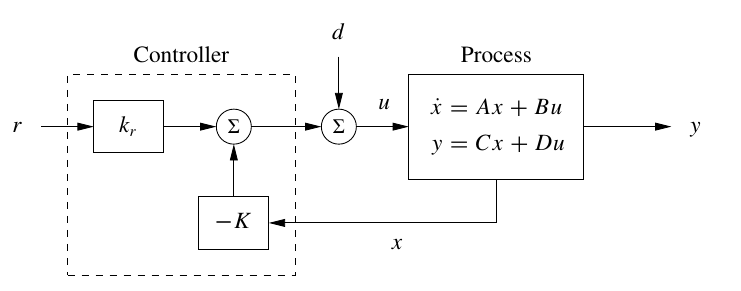
\includegraphics[scale=0.280]{img/state_feedback/state_feedback_sys.jpeg}
\end{center}
\caption{A feedback control system with state feedback. The controller uses the system
state $x$ and the reference input $r$ to command the process through its input $u$. We model
disturbances via the additive input $d$.}
\label{state_feedback_sys_II}
\end{figure}

The full system consists of the process dynamics, which we take to be linear, the controller
elements $K$ and $k_r$ , the reference input (or command signal) $r$ and process disturbances $d$. The goal of the feedback controller is to regulate the output of the system $y$ such that it tracks the reference input in the presence of disturbances and also uncertainty in the process dynamics.

An important element of the control design is the performance specification.
The simplest performance specification is that of stability: in the absence of any
disturbances, we would like the equilibrium point of the system to be asymptotically
stable. More sophisticated performance specifications typically involve giving desired properties of the step or frequency response of the system, such as specifying the desired rise time, overshoot and settling time of the step response. Finally, we are often concerned with the disturbance attenuation properties of the system: to
what extent can we experience disturbance inputs $d$ and still hold the output $y$ near the desired value?

Consider a system described by the linear differential equation



\begin{equation}
\frac{dx}{dt} = Ax + Bu ~~ y = Cx + Du
\end{equation}


\section{Exercises}

\textbf{Exercise 1}

Consider the system 

\begin{eqnarray}
\dot{x} = Ax + Bu \\
y = Cx 
\end{eqnarray}

controlled by a state feedback controller: 

\begin{equation}
 u = -Kx  
\end{equation}

What are  the sizes of the matrices A, B, C, and K if we have one input signal, three states and two output signals.

\textbf{Answer}

Since the state has three components then $A$ must be $3\times 3$. As we have only one input but the result of $Bu$ must be added to the result of $Ax$ then $B$ must be $3\times 1$.
Since the output has two components then $C$ must be $2\times 3$. Finally, $K$ must be $1\times 3$.

\textbf{Exercise 2}

Consider again the system in the previous  question. Assume now that but now the system has two input signals, three states and one output signal. What are the sizes of the involved matrices?

\textbf{Answer}

Using the same line of reasoning, since the state has three components then $A$ must be $3\times 3$. As we have only two input but the result of $Bu$ must be added to the result of $Ax$ then $B$ must be $3\times 2$. Since the output has two components then $C$ must be $1\times 3$. Finally, $K$ must be $2\times 3$.


\textbf{Exercise 3}

Consider again the system in the previous  question. Assume now that but now the system has two input signals, four states and one output signal. What are the sizes of the involved matrices?

\textbf{Answer}

Using the same line of reasoning, since the state has three components then $A$ must be $4\times 4$. As we have only two input but the result of $Bu$ must be added to the result of $Ax$ then $B$ must be $4\times 2$. Since the output has two components then $C$ must be $1\times 4$. Finally, $K$ must be $2\times 4$.



\textbf{Exercise 4}

Consider the mechanical system shown in Figure \ref{Mechanical_system_3_1_1_ex_4} 


\begin{figure}[!htb]
\begin{center}

\includegraphics[scale=0.280]{img/state_feedback/Mechanical_system_3_1_1_ex_4.png}
\end{center}
\caption{Schematic of mechanical system}
\label{Mechanical_system_3_1_1_ex_4}
\end{figure}

The system is described by the following state-space model

\begin{eqnarray}
\begin{bmatrix}
 \dot{x}_1 \\
 \dot{x}_2 
\end{bmatrix} =  
\begin{bmatrix}
 0 & 1 \\
 0 & -c/m
\end{bmatrix}
\begin{bmatrix}
 x_1 \\
 x_2  
\end{bmatrix}+
\begin{bmatrix}
 0 \\
 1/m  
\end{bmatrix}u \\
y =
\begin{bmatrix}
 1 & 0 
\end{bmatrix}
\begin{bmatrix}
 x_1 \\
 x_2  
\end{bmatrix}
\end{eqnarray}

where $x_1$ is the position of the mass, $x_2$ is the velocity of the mass and $u$ is the input signal, the force. The output $y$ is the position. Assume that the desired closed loop characteristic polynomial is

\begin{equation}
p(s) = s^2 + 2\zeta \omega_n s +\omega_{n}^{2}  
\end{equation}

and the state feedback controller is 

\begin{equation}
u = -Kx  
\end{equation}

Determine the elements of $K=[k_{11}, k_{12}]$

\textbf{Answer}

By substituting the expression for $u$ into the equation describing the state dynamics, we can write

\begin{equation}
\dot{x} = (A - BK)x
\end{equation}

We can now calculate the characteristic polynomial via


\begin{equation}
det(s I - (A - BK)) = 0
\end{equation}

This gives us a second order polynomial

\begin{equation}
s^2 + ((c + k_{12})/m)s + k_{11}/m
\end{equation}

by matching the coefficients with the desired closed loop characteristic polynomial, we get

\begin{equation}
k_{12} = 2 \zeta m\omega_{n} -c, ~~ k_{11} = m \omega_{n}^{2}
\end{equation}



\textbf{Exercise 5}

Consider the mechanical system shown in Figure \ref{Mechanical_system_3_1_1_ex_4} described by the same steady-state model. Assume that the feedback controller is

\begin{equation}
u = -Kx + K_r r 
\end{equation} 

where $r$ is the reference signal. We want to determine the steady state reference gain $K_r$ such that the steady-state level is 1.

\textbf{Answer}

The reference gain $K_r$ is given by 

\begin{equation}
K_r = - ( C(A-BK)^{-1}B)^{-1} 
\end{equation}


\textbf{Exercise 6}

Consider the closed loop system with the controller designed as in the previous exercise. Determine the transfer function for closed loop system, from the reference signal to the output


\textbf{Exercise 2}

The linearized longitudinal vehicle dynamics model for a vehicle traveling at $20 m/sec$ on a flat road is given by the following state-space model


\begin{eqnarray}
\begin{bmatrix}
 \dot{x}_1\\
 \dot{x}_2
\end{bmatrix}= 
\begin{bmatrix}
 -1.25 & 0 \\
 0.000005 & -0.0024 
\end{bmatrix}
\begin{bmatrix}
 x_1\\
 x_2
\end{bmatrix} +  
\begin{bmatrix}
 20000\\
 0
\end{bmatrix}u +
\begin{bmatrix}
 0\\
 -9.82
\end{bmatrix}d_1 \\
y=
\begin{bmatrix}
 0 & 1  \\
\end{bmatrix}
\begin{bmatrix}
 x_1\\
 x_2
\end{bmatrix} 
\end{eqnarray}

where $x_1$ is the force at the wheels, $x_2$ is the vehicle velocity, $u$ is the input signal and $d_1$ is the disturbance of the road.

Design a state feedback cruise controller using pole placement on the form

\begin{equation}
u = - K x + k_r r
\end{equation}

such that the closed loop system's characteristic polynomial becomes 
\begin{equation}
p(s) = s^2 + 2\zeta \omega_n s +\omega_{n}^{2}  
\end{equation}

where $\omega_n=0.6$ and $\zeta = 1/\sqrt{2}$. The reference gain $k_r$ should be chosen such that the steady state gain is 1. The disturbance $d_1$ can be considered to be 0.

